\chapter{Solid state chemistry}
\section{Preliminary}
\subsection{Bravais lattices}
\subsubsection{Definitions}
We establish definitions below.
\begin{defi}[Bravais cystal lattice]
The \emph{Bravais cystal lattice} is one way to describe crystal lattices, as a translationally periodic array of indistinguishable mathematical points called the \emph{lattice points}. These lattice points are generated by \emph{primitive lattice vectors} (see below).
\end{defi}
\begin{defi}[Lattice motif or basis]
The lattice points are not, in general, the positions of the atoms or molecules that constitute the physical lattice, however, they are imagined to be identically attached to each of the lattice points in a \emph{motif} or \emph{basis}. The motif can be a single atom, a pair of ions (say with one on the lattic point and one a fixed translation away) and so on.
\end{defi}
\begin{defi}[Lattice vectors]
\emph{Lattice vectors} are any vectors connecting one lattice point with another.
\end{defi}
\begin{defi}[Primitive lattice vectors]
\emph{Primitive lattice vectors} can generate the whole lattice by starting at an arbitrary starting lattice point and move by integer multiples of these vectors. These define the edges of \emph{primitive unit cells}.
\end{defi}
\begin{defi}[Unit cells]
Any non-collinear lattice vectors can define the edges of a \emph{unit cell}. These are \emph{not unique}. They are said to tessellate the entire lattice.
\end{defi}
\begin{defi}[Lattice point count]
A unit cell can contain any number of lattice point. They are imagined as `pies' that are cut by the edges, or wholly contained by the cell. For example, a vertex of a cube on the lattice point will account for $\frac{1}{8}$ of a lattice point and an edge point will account for $\frac{1}{4}$ of a lattice point.
\end{defi}
\begin{defi}[Primitive unit cells]
\emph{Primitive unit cells} are unit cells that contain just one lattice point. These are also \emph{not unique}. 
\end{defi}
\subsubsection{Types of Bravais lattices}
\label{bravaistypes}
There are 14 possible Bravais lattices in three dimensions. They are classed first by their lattice systems, which contains requirements for the three lattice angles, the three cell edge lengths (not necessarily primitive lattice vector lengths unless the lattice is primitive), and the symmetry requirements.\par
Each lattice system can give rise to a maximum of 4 unit cell types:
\begin{enumerate}
	\item \textbf{Primitive} (\textbf{P}): Unit cell formed by primitive lattice vectors therefore has a lattice point at each corner.
	\item \textbf{Body-centered} (\textbf{I}): Primitive with one lattice point at the centre of the cell.
	\item \textbf{Face-centered} (\textbf{F}): Primitive with one lattice point at the centre of each face.
	\item \textbf{Base-centered} (\textbf{C}): Face-centered but with lattice points at the center of only one pair of opposing faces, which are conventionally oriented to be the base.
\end{enumerate}
We are only going to look at the cubic lattice system, which says $\alpha=\beta=\gamma=90^{\circ}$ and $a=b=c$, and requires the symmetry of at least four threefold axes at $109^{\circ}28'$ (the tetrahedral angle) to each other. The symmetry requirement excludes the base-centered unit cell type. We have three left to study in detail.
\subsubsection{The cubic lattices}
\paragraph{Simple cubic (cubic P)} 
The unit cell is just a cube with lattice points at the corners, with side length $a$, the primitive lattice vectors are 
\begin{equation*}
	\bvec{a}_1=a(1,0,0)\ \ \bvec{a}_2=a(0,1,0)\ \ \bvec{a}_3=a(0,0,1)\ \ V_c=a^3
\end{equation*}
\emph{Packing fraction}\\
Imagine spheres centered at the lattice points and they keep expanding until they just touch each other - in this case the spheres on the edges will touch first with $r=\frac{a}{2}$. This means the packing fraction, $\rho$, of primitive cubic is
\begin{equation}
	\rho=\frac{V_{\mathrm{spheres}}}{V_{\mathrm{cell}}}=\frac{\tfrac{4}{3}\pi r^3}{a^3}=\frac{\tfrac{4}{3}\pi(\tfrac{a}{2})^3}{a^3}=\frac{\pi}{6}\approx52\%
\end{equation}
\paragraph{Body-centered cubic (cubic I)} 
The unit cell that's easiest to picture and work with is a non-primitive unit cell that was described in \cref{bravaistypes}. The primitive vectors and unit cell volumes are 
\begin{equation*}
	\bvec{a}_1=\tfrac{1}{2}a(1,1,-1)\ \ \bvec{a}_2=\tfrac{1}{2}a(-1,1,1)\ \ \bvec{a}_3=\tfrac{1}{2}a(1,-1,1)\ \ V_c=\tfrac{1}{2}a^3
\end{equation*}
\emph{Packing fraction}
The spheres along the body diagonal touch first and is equal to 4 radii. The length of the body diagonal is $\sqrt{3}a=3r$, so $a=4r/\sqrt{3}$. There are 2 spheres contained in the unit cell considered, whose volume is $a^3$. The packing fraction is then given as
\begin{equation}
 	\rho=\frac{V_{\mathrm{spheres}}}{V_{\mathrm{cell}}}=\frac{2\times\tfrac{4}{3}\pi r^3}{a^3}=\frac{2\times\tfrac{4}{3}\pi r^3}{(4r/\sqrt{3})^3}=\frac{\sqrt{3}\pi}{8}\approx68\%
\end{equation} 
\paragraph{Face-centered cubic (cubic F)} 
The unit cell is again non-primitive. The primitive lattice vectors and volume of primitive unit cell are
\begin{equation}
	\bvec{a}_1=\tfrac{1}{2}a(1,1,0)\ \ \bvec{a}_2=\tfrac{1}{2}a(0,1,1)\ \ \bvec{a}_3=\tfrac{1}{2}a(1,0,1)\ \ V_c=\tfrac{1}{4}a^3
\end{equation}
\emph{Packing fraction}
In this case the spheres on the face diagonals touch first and is equal to 4 radii. The length of the face diagonal is $\sqrt{2}a$, so $a=4r/\sqrt{2}$. The unit cell contains 4 spheres. The packing fraction is therefore
\begin{equation}
	\rho=\frac{V_{\mathrm{spheres}}}{V_{\mathrm{cell}}}=\frac{4\times\tfrac{4}{3}\pi r^3}{(4r/\sqrt{2})^3}=\frac{\pi}{3\sqrt{2}}\approx74\%
\end{equation}
This is the greatest packing density possible. Therefore the cubic face-centered lattice is also known as \emph{cubic close-packed}. 
\subsubsection{Lattices with a motif}
Consider a face-centered cubic lattice, with sodium ions on the lattice points, and chloride ions $(0,0,\tfrac{1}{2}a)$ away. A pair of sodium and chloride ions forms the motif for the archetypal \ch{NaCl} lattice.
\subsection{The ionic model}
\subsubsection{The model}
Consider now a 1-D array of alternating negative and positive charges with $z_-$ and $z_+$ charges respectively, spaced $a$ apart. Starting arbitrarily from a positive charge and consider it the origin, looking to the right, the net electrostatic interaction is
\begin{equation}
	-\frac{z_+z_-e^2}{4\pi\ep_0 a}+\frac{z_+z_-e^2}{4\pi\ep_0 (2a)}-\frac{z_+z_-e^2}{4\pi\ep_0 (3a)}+\dots
\end{equation}
Now looking left as well and multiplying by the Avogadro's number we have
\begin{equation}
\begin{aligned}
	E_{\mathrm{electrostatic}}&=-2N_A\frac{z_+z_-e^2}{4\pi\ep_0 a}(1-\tfrac{1}{2}+\tfrac{1}{3}+\dots)\\
	&=-2\ln2N_A\frac{z_+z_-}{4\pi\ep_0 a}\\
	&\equiv-\mathcal{A}N_A\frac{z_+z_-e^2}{4\pi\ep_0 a}
\end{aligned}
\end{equation}
where $\mathcal{A}=2\ln2$ is the \emph{Madelung constant}, specific to each lattice under consideration.\par
However this presents the problem that the interaction energy is always attractive and predicts lattice collapse. An \emph{ansatz} repulsion term $B/a^n$ has to be introduced, corresponding to quantum mechanical repulsion between filled orbitals. The order $n$ (typically 9 or greater) is fitted \emph{post-hoc} from experimental data on equilibrium lattice spacing, and the constant $B$ can be eliminated as we will show below. The total energy as a function of lattice spacing $a$ is written as
\begin{equation}
	E(a)=-\frac{N_A\mathcal{A}z_+z_-e^2}{4\pi\ep_0a}+\frac{B}{a_n}
\end{equation}
At equilibrium, $\diff{E}/{a}=0$ and $a=a_0$, we can write
\begin{equation}
	\frac{nB}{a_0^{n+1}}=\frac{N_A\mathcal{A}z_+z_-e^2}{4\pi\ep_0a_0^2}
\end{equation}
which means we can eliminate $B$ by multiplying $a_0/n$ throughout:
\begin{equation}
	\frac{B}{a_0^n}=\frac{N_A\mathcal{A}z_+z_-e^2}{4\pi\ep_0a_0n}
\end{equation}
So the equilibrium energy is
\begin{equation}
	E_0=-\frac{N_A\mathcal{A}z_+z_-e^2}{4\pi\ep_0a_0} \lf(1-\frac{1}{n}\rt)
\end{equation}
To get an approximation for lattice energy, which involves the process of
\begin{equation*}
	\ch{MX (s) -> M+ (g) + X- (g)}
\end{equation*}
we assume that infinitely separated ions have zero energy, and so $\Delta U=-E_0$, and under such a simplistic model is it acceptable to approximate $\Delta H\approx\Delta U$, so
\begin{thrm}[Lattice energy]
The lattice energy arising from the ionic model is given as
\begin{equation}
	\Delta_L H^{\circ}\approx\frac{N_A\mathcal{A}z_+z_-e^2}{4\pi\ep_0a_0} \lf(1-\frac{1}{n}\rt)
\end{equation}
\end{thrm}
The Madelung constant for different lattices are given below
\begin{center}
	\begin{tabular}{cccc}
	\hline
	lattice & example & coordination & $\mathcal{A}$\\
	\hline
	caesium chloride & \ch{CsCl} & 8:8 & 1.763\\
	fluorite & \ch{CaF2} & 8:4 & 2.519\\
	rock salt & \ch{NaCl} & 6:6 & 1.748\\
	rutile & \ch{TiO2} & 6:3 & 2.408\\
	sphalerite & \ch{ZnS} & 4:4 & 1.638\\
	\hline
	\end{tabular}
\end{center}
\subsubsection{Radius ratios}
It is not always possible for the ions to touch if say the cations are very large, \ch{Cs+} for example and the anion is very small, \ch{F-} for example, the cations will touch first before the anions can touch the cation \emph{optimally}, meaning doing so while it still resides on the motif points. If this happens the lattice energy is not as large as it can be, and a different lattice may be adopted to allow closest approch of the ions. \par
We can work out the lowest value of $r_+/r_-$ for each lattice type:\\
\paragraph{Rock salt} 
We can work out the minimum radius ratio by drawing out the limiting scenario:
\begin{center}
	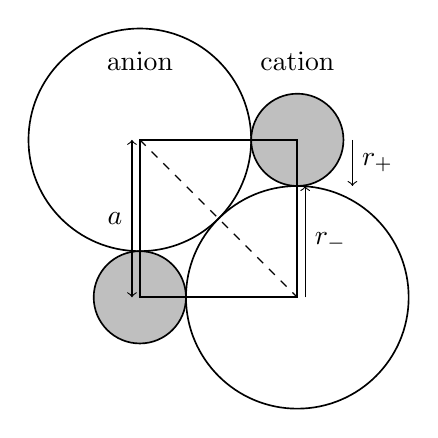
\begin{tikzpicture}
	\draw[fill=lightgray,semithick] (0,-2) circle (0.586cm);
	\draw[fill=lightgray,semithick] (2,0) circle (0.586cm);	
	\draw[semithick] (0,0) circle (1.414cm);
	\draw[semithick] (2,-2) circle (1.414cm);
	\node at (0,1) {anion};
	\node at (2,1) {cation};
	\draw[semithick] (0,0) rectangle (2,-2);
	\draw[thin,dashed] (0,0) -- (2,-2);
	\draw[<->] (-0.1,0) -- (-0.1,-2);
	\node[left] at (-0.1,-1) {$a$};
	\draw[->] (2.1,-2) -- (2.1,-0.586);
	\node[right] at (2.1, -1.293) {$r_-$};
	\draw[->] (2.7,0) -- (2.7,-0.586);
	\node[right] at (2.7,-.293) {$r_+$};
\end{tikzpicture}
\end{center}
in which the diagonal $\sqrt{2}a=2r_-$, and $a=r_-+r_+$, so we can conclude that
\begin{equation}
	\frac{r_+}{r_-}=\frac{a-\sqrt{2}a/2}{\sqrt{2}a/2}=\sqrt{2}-1\approx0.414
\end{equation}
The minimum radius ratios for other lattice types have been worked out:
\begin{center}
	\begin{tabular}{cccc}
	\hline
	lattice  & coordination & minimum radius ratio &$\mathcal{A}$\\
	\hline
	caesium chloride & 8:8 & 0.732 & 1.763\\
	rock salt & 6:6 & 0.414 & 1.748\\
	sphalerite & 4:4 & 0.225 & 1.638\\
	\hline
	\end{tabular}
\end{center}
Keeping in mind that $E\propto\mathcal{A}$, the lattice would like to keep the lattice energy as high as possible while maintaining maximum contact. For example, for \ch{MgO}, $r_+/r_-\approx0.51$, which is too small for the caesium chloride structure. So it can `choose' either rock salt of sphalerite. As rock salt has higher Madelung constant, it should be preferred, and is indeed the case.
\section{Free-electron gas model}
\subsection{Unconstrained FEG}
\subsubsection{One-dimensional FEG}
This model assumes that electrons do not interact with each other or the nuclei. Essentially they are treated as unconstrained gas molecules. In one dimension, the \sch equation was solved in \cref{freepart}, with 
\begin{equation}
	\hat{H}=-\frac{\hbar^2}{2m_e}\diff[2]{}{x}
\end{equation}
so the \sch reads
\begin{equation}
	-\frac{\hbar^2}{2m_e}\diff[2]{\psi}{x}=E\psi\ \ \imp\ \ \diff[2]{\psi}{x}=-k^2\psi
\end{equation}
where $k=\frac{2m_eE}{\hbar}$ or $E_k=\hbar^2k^2/2m_e$, the time-dependent solution is 
\begin{equation}
	|\ups_k(x,t)\rgl=Ae^{i(kx-\hbar k^2t/2m)}
\end{equation}
with momentum
\begin{equation}
	\hat{p}|\ups_k\rgl=\hbar k
\end{equation}
The wavelength can be defined as distance before the phase is reset, so in this case
\begin{equation}
	\lambda=\frac{2\pi}{|k|}
\end{equation}
\subsubsection{Three-dimensional FEG}
In three dimensions, the solution is 
\begin{equation}
	|\ups_{\bvec{k}}(\bvec{r},t)\rgl=Ae^{i\bvec{k}\cdot\bvec{r}-\hbar |\bvec{k}|^2t/2m}
\end{equation}
where
\begin{equation}
	E_{\bvec{k}}=\frac{\hbar^2|\bvec{k}|^2}{2m_e}
\end{equation}
and the momentum is
\begin{equation}
	\bvec{p}=\hbar\bvec{k}
\end{equation}
and the wavelength is
\begin{equation}
	\lambda=\frac{2\pi}{|\bvec{k}|}
\end{equation}
Now we need to introduce the important concept of 
\begin{defi}[$k$-space]
As the three-dimensional wavefunctions are defined uniquely by the wavevector $\bvec{k}$, these wavevectors can be thought to correspond to a point in the $k$-space. The squared distance from the origin is proportional to energy.
\end{defi}
\subsection{Quantization}
The unconstrained systems above are, of course, not quantised, which is a major problem. We must introduce some sort of boundary condition:
\begin{thrm}[The Born von Karman boundary conditions]
\label{fegbvk}
The BvG boundary conditions posits that the two edges of the crystals are condinuous, \ie
\begin{equation}
	\ups(\bvec{r},t)=\ups(\bvec{r}+L_i\bvec{a}_i,t)
\end{equation}
where $L_i$ is the number of cells in the $\bvec{a}_i$ direction. In effect, it requires that
\begin{equation}
	kL_1a_i=2n_1\pi\ \ \imp\ \ k=n_1\lf(\frac{2\pi}{L_1a_1} \rt)
\end{equation}
\end{thrm}
\paragraph{Justification of BvK boundary condition}
There are two ways to introduce boundary conditions:
\begin{itemize}
	\item Particle-in-a-box boundary conditions (linear wire)
	\item BvK boundary conditions (circular wire)
\end{itemize}
The table below compares the two boundary conditions
\begin{center}
	\begin{tabular}{r|l|l}
	\hline
	& Linear wire & Circular wire\\
	\hline
	Boundary conditions & $kL=n\pi$, $n\in\mathbb{Z}^+$ & $kL=2n\pi$, $n\in\mathbb{Z}$\\
	Energies & $E_n=\hbar^2\pi^2n^2/2mL^2$ & $E_n=4\hbar^2\pi^2n^2/2mL^2$\\
	Eigenfunctions & $A\sin(n\pi x/L)$ & $B\exp(2ni\pi x/L)$\\
	\hline
	\end{tabular}
\end{center}
Basically, the energy levels for the two models look like this
\begin{center}
	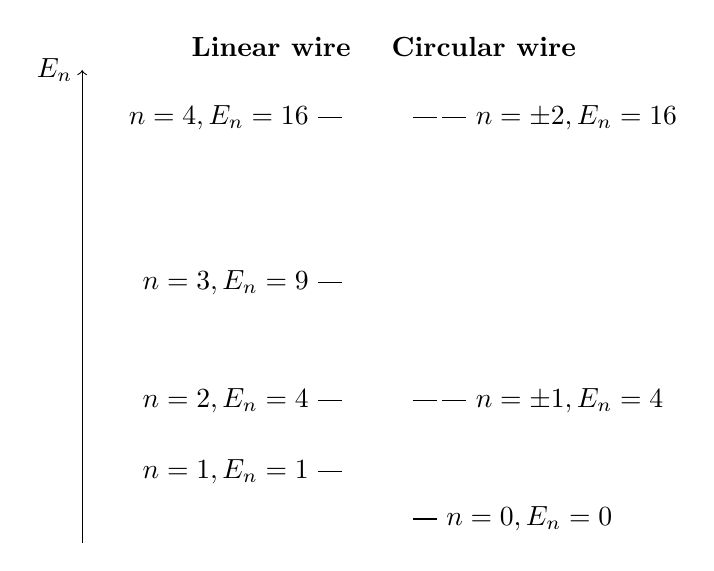
\begin{tikzpicture}[scale=0.3]
	\node at (-2,19){\textbf{Linear wire}};
	\node at (7,19){\textbf{Circular wire}};
	\draw[->] (-10,-2) -- (-10,18) node [anchor=east] {$E_n$};
	\draw (0,1)node[anchor=east] {$n=1,E_n=1$} -- (1,1);
	\draw (0,4)node[anchor=east] {$n=2,E_n=4$} -- (1,4);
	\draw (0,9)node[anchor=east] {$n=3,E_n=9$} -- (1,9);
	\draw (0,16)node[anchor=east] {$n=4,E_n=16$} -- (1,16);
	\draw (4,-1) -- (5,-1)node[anchor=west]{$n=0,E_n=0$};
	\draw (4,4) -- (5,4);
	\draw (5.25,4) -- (6.25,4)node[anchor=west]{$n=\pm1,E_n=4$};
	\draw (4,16) -- (5,16);
	\draw (5.25,16) -- (6.25,16)node[anchor=west]{$n=\pm2,E_n=16$};
\end{tikzpicture}
\end{center}
And in the limit that $N\rightarrow\inf$, the density of states is approximately the same, and also the HOMO, now Fermi level, is also the same.\par
So what's different? The reason for choosing the circular wire is threefold:
\begin{enumerate}
	\item The eigenfunctions of the linear wire are not eigenfunctions of the momentum operator, while the circular wire ones are, yielding $\hbar\bvec{k}$ naturally.
	\item By ignoring the surface effects, the boundary conditions of the linear wire do not arise as there's no `outside' where $V(x)=\inf$.
	\item The circular wire allows potential energy functions of symmetry $V(x+N\bvec{a})=V(x)$, while the linear wire does not. This is important in the full theory.
\end{enumerate}
Simply put, the crystal is imagined to be infinite so that the edge effects are ignored. \par
In the $k$-space, the allowed wavefunctions (states) are just a series of points spaced $2\pi/L_1a_1$ apart. The density of BvK allowed states in 1D is therefore
\begin{equation}
	\frac{L_1a_1}{2\pi}\equiv\frac{\mathcal{L}}{2\pi}
\end{equation}
where $\mathcal{L}=L_1a_1$ is called the BvK length.\par
In two and three dimensions the density of BvK allowed states are readily generalised to
\begin{equation}
\begin{aligned}
&\text{2D: }\frac{L_1L_2A_c}{(2\pi)^2}\equiv\frac{\mathcal{A}}{(2\pi)^2}\\
&\text{3D: }\frac{L_1L_2L_3V_c}{(2\pi)^2}\equiv\frac{\mathcal{V}}{(2\pi)^3}
\end{aligned}
\end{equation}
\subsection{Fermi-Dirac distribution}
The Maxwell-Boltzmann distribution assumes that the particles are distinguishable and any number of particles can occupy a level. However that is clearly not applicable to electrons, which are fermions. The Pauli exclusion principle states that two of more \emph{identical fermions} cannot occupy the same quantum state. A distribution adhering to the Pauli exclusion principle is the 
\begin{thrm}[Fermi-Dirac distribution]
The distribution states that the average number of fermions in a single-particle state $i$ is given by
\begin{equation}
	\lgl n_i\rgl=\frac{1}{\exp[(\ep_i-\mu)/kT]+1}
\end{equation}
where we can write $\lgl n_i\rgl$ as $f(\ep_i)$, and approximate the chemical potential $\mu$ with the \emph{Fermi energy}, $\ep_{\mathrm{F}}$, to give
\begin{equation}
	f(\ep_i)=\frac{1}{\exp[(\ep_i-\ep_{\mathrm{F}})/kT]+1}
\end{equation}
\end{thrm}
\begin{figure}[ht]
	\centering
	\includegraphics[width=8cm]{fermilevels}
	\caption{Comparison between the predictions of Fermi-Dirac and Maxwell-Boltzmann distributions}
	\label{fig:fermilevels}
\end{figure}
The result is a logistic function ranging from 1 for energies much lower than the Fermi level to 0 for energies much higher than the Fermi level. Raising the temperature has the effect of exciting particles near the Fermi level, `blurring' the distribution:
\begin{figure}[ht]
	\centering
	\includegraphics[width=8cm]{fermigraph}
	\caption{The blurring of the Fermi-Dirac distribution occurs at higher temperautres. Notice it always runs from 1 to 0, as required by the Pauli exclusion principle.}
	\label{fig:fermigraph}
\end{figure}
\begin{defi}[Fermi quantities]
The \emph{Fermi energy} is defined only at 0 K, which is defined as the highest filled level at 0K.\par
The \emph{Fermi level}, $E_{\mathrm{F}}$ is the energy level correponding to Fermi energy, but remains defined for all temperatures.\par
The \emph{Fermi wavevector}, $\bvec{k}_{\mathrm{F}}$ is the wavevector corresponding to the Fermi level.\par
Alternatively, the Fermi level can be approximately seen to be the energy level that has half occupancy at non-zero temperatures.
\end{defi}
\subsection{Properties of the FEG}
\subsubsection{Density of states}
The density of BvK states in 3D is 
\begin{equation}
	W(E)=\underbrace{\vphantom{\frac{\mathcal{V}}{(2\pi)^3}} \frac{4}{3}\pi|\bvec{k}|^3}_{\mathrm{`volume'}}\times\underbrace{\frac{\mathcal{V}}{(2\pi)^3}}_{\mathrm{density}}
\end{equation}
and we know that
\begin{equation}
	|\bvec{k}|=\lf(\frac{2m_eE}{\hbar^2} \rt)^{\frac{1}{2} }
\end{equation}
Keeping in mind that we although each level can accept only one \emph{identical} Fermion, electrons have two spin states and they spin-pair so each level can be doubly occupied, so a factor of two is applied in front:
\begin{equation}
	W(E)=2\times\frac{4}{3}\pi|\bvec{k}|^3\times\frac{\mathcal{V}}{(2\pi)^3}=\frac{|\bvec{k}|^3\mathcal{V}}{3\pi^2}=\frac{\mathcal{V}}{3\pi^2}\lf(\frac{2m_eE}{\hbar^2} \rt)^{\frac{3}{2}}
\end{equation}
Density of states soon follows by simple differentiation
\begin{thrm}[Density of BvK states]
The number of BvK states with energy up to $E$ is given as
\begin{equation}
	W(E)=\frac{\mathcal{V}}{3\pi^2}\lf(\frac{2m_eE}{\hbar^2} \rt)^{\frac{3}{2}}
\end{equation}
so the density of states is given as
\begin{equation}
	D(E)=\diff{W(E)}{E}=\frac{\mathcal{V}}{2\pi^2}\lf(\frac{2m_e}{\hbar^2} \rt)^{\frac{3}{2}}E^{\frac{1}{2}}
\end{equation}
We note that the density of states increase with energy.
\end{thrm}
\subsubsection{Fermi quantities}
Suppose that the number density of electrons in the metal is $n_e$, so there are $n_e\mathcal{V}$ electrons in the BvK volume. At absolute zero, where Fermi energy is defined, we can say that the number of states filled are equal to the number of electrons\footnote{Although we commonly think of the levels as being doubly filled, for the formalism of the BvK we think of two degenerate levels at the same energy, one for the spin up electron one for the spin down.}, which is to say
\begin{equation}
	W(E_{\mathrm{F}})=n_e\mathcal{V}
\end{equation}
so
\begin{equation}
\begin{aligned}
	&\frac{\mathcal{V}}{3\pi^2}\lf(\frac{2m_eE_{\mathrm{F}}}{\hbar^2} \rt)^{\frac{3}{2}}=n_e\mathcal{V}\\
	\imp&E_{\mathrm{F}}=\lf(\frac{\hbar^2}{2m_e} \rt)(3\pi^2n_e)^{3/2}
\end{aligned}
\end{equation}
And the Fermi wavevector can also be worked out:
\begin{equation}
	|\bvec{k}|_{\mathrm{F}}=(3\pi^2n_e)^{1/3}
\end{equation}
To summarise
\begin{thrm}[Fermi level and wavevector]
For a metal with eletron density $n_e$, the Fermi level and Fermi wavevector are given as
\begin{equation}
\begin{aligned}
&E_{\mathrm{F}}=\lf(\frac{\hbar^2}{2m_e} \rt)(3\pi^2n_e)^{3/2}\\
&|\bvec{k}|_{\mathrm{F}}=(3\pi^2n_e)^{1/3}
\end{aligned}
\end{equation}
\end{thrm}
\subsubsection{Average energy}
At absolute zero the average energy is
\begin{equation}
	\lgl E\rgl=\frac{\text{total energy}}{\text{number of states}}=\frac{\int^{E_\text{F}}_0E\times D(E)\dif E}{\int^{E_\text{F}}_0D(E)\dif E}
\end{equation}
The integrals are straightforward and the result is 
\begin{thrm}[Average energy at absolute zero]
The Fermi-Dirac distribution predicts that for a free electron gas, the average energy at absolute zero is
\begin{equation}
	\lgl E\rgl=\frac{3}{5}E_{\mathrm{F}}
\end{equation}
\end{thrm}
\subsubsection{Heat capacity}
Assuming that the metal atom has only 1 valence electron, one mole of the metal contains $N_A$ valence electrons. To a crude approximation, the number of excited electrons (those within $kT$ of Fermi level) is
\begin{equation}
	n=N_A\times\frac{kT}{E_{\mathrm{F}}}=\frac{RT}{E_{\mathrm{F}}}
\end{equation}
Again, to an approximation, these electrons on average has $kT$ more in energy\footnote{They already had some intrinsic kinetic energy as a consequence of the Fermi-Dirac distribution, and now they have an additional $kT$ in `thermal' energy, which is just additional kinetic energy.}, so the total increase in energy as a result of raised temperature is
\begin{equation}
	\Delta U=kT\frac{RT}{E_{\mathrm{F}}}\equiv\frac{R}{T_{\mathrm{F}}}T^2
\end{equation}
where $T_{\mathrm{F}}=E_{\mathrm{F}}/k$ is the \emph{Fermi temperature}, so the heat capacity is roughly
\begin{equation}
	C_{V,m}=\frac{2R}{T_{\mathrm{F}}}\times T
\end{equation}
This treatment gives poor agreement with data, as the estimation of the number of electrons is poor and does not take into account the density of states. A more sophisticated treatment gives
\begin{equation}
	C_{V,m}=\frac{\pi^2RT}{2T_{\mathrm{F}}}
\end{equation}
\subsubsection{Bulk modulus}
The bulk modulus is the ratio between the pressure change and the fractional change in volume, which, in calculus terms is
\begin{equation}
	B=-V\diffp pV[T,N]
\end{equation}
Also the definition of pressure in terms of the internal energy is
\begin{equation}
	p=-\diffp UV[N]
\end{equation}
At absolute zero, we know the average energy, so the internal energy is
\begin{equation}
	U=N\lgl E\rgl=\frac{3}{5}NE_{\mathrm{F}}
\end{equation}
The Fermi energy is
\begin{equation}
	E_{\mathrm{F}}=\lf(\frac{\hbar^2}{2m_e} \rt)(3\pi^2n_e)^{2/3}
\end{equation}
The electron number density, in the formalism of BvK is just 
\begin{equation}
	n_e=\frac{N}{\mathcal{V}}
\end{equation}
So we can write 
\begin{equation}
	U=\frac{3}{5}N\underbrace{\lf(\frac{\hbar^2}{2m_e} \rt)(3\pi^2N)^{2/3}}_{c}\mathcal{V}^{-2/3}
\end{equation}
So 
\begin{equation}
	p=\frac{2}{5}Nc\mathcal{V}^{-5/3}
\end{equation}
and the bulk modulus is
\begin{equation}
	B=\frac{2}{3}Nc\mathcal{V}^{-5/3}
\end{equation}
Since $E_{\mathrm{F}}=c\mathcal{V}^{-2/3}$, we can finally write
\begin{equation}
	B=\frac{2}{3}E_{\mathrm{F}}N/\mathcal{V}=\frac{2}{3}E_{\mathrm{F}}n_e
\end{equation}
\subsubsection{Electrical conductivity}
The `ground state' of a 2-dimensional FEG in the $k$-space at 0 K will show occupied $k$-states within a circle of radius $|\bvec{k}|$ centred at $(0,0)$, as the highest occupied level is the Fermi level (at 0 K), and the momentum given by $\hbar\bvec{k}$ is on average zero. The circle is called the \emph{Fermi circle}.\par
Now after the application of an electric field along the $x$-direction, the average momentum will be in the $x$-direction\footnote{It is not infinite because electrons are scattered so a steady-state \emph{drift velocity} is reached.}, so the centre of the Fermi circle will be shifted to the right.\par
It is important to note that the only reason conduction can happen is because there are vacant states just outside the Fermi circle.\par
A simple model that can give us the conductivity is the
\begin{thrm}[The Drude model]
The Drude model says that the drift velocity, $v_{\mathrm{d}}$ is given by
\begin{equation}
	v_{\mathrm{d}}=e\mathcal{E}\tau/m_{\mathrm{e}}
\end{equation}
\end{thrm}
\begin{proof}
	The net acceleration experienced by the electron due to the field is $e\mathcal{E}/m_{\mathrm{e}}$. Supposing that the average time between collisions is $\tau$, which knocks the speed down to zero again, the average velocity is just accleration times time, which gives the result required.
\end{proof}
The current density is defined as the charge per unit time per unit area, which can be written as
\begin{equation}
	j=\frac{n_{\mathrm{e}}v_{\mathrm{d}}\Delta tAe}{\Delta tA}=n_{\mathrm{e}}v_{\mathrm{d}}e=n_{\mathrm{e}}e^2\mathcal{E}\tau/m_{\mathrm{e}}
\end{equation}
The Ohm's law says that 
\begin{equation}
	j=\sigma\mathcal{E}
\end{equation}
so we can extract
\begin{equation}
	\sigma=n_{\mathrm{e}}e^2\tau/m_{\mathrm{e}}
\end{equation}
The \emph{electron mobility}, $\mu_{\mathrm{e}}$ (not magnetic susceptibility) is 
\begin{equation}
	\mu_{\mathrm{e}}\equiv\frac{v_{\mathrm{d}}}{\mathcal{E}}=\frac{e\tau}{m_{\mathrm{e}}}
\end{equation}
\subsection{The nearly-free electron gas}
\subsubsection{Failure of the FEG and Brillouin zones}
The free electron gas assumes no interactions whatsoever with the underlying lattice, which is of course not true. The FEG model notably fails when the wavefunctions $\psi_{\bvec{k}}$ are diffracted by the lattice. To take this into account, the Brillouin zone is defined:
\begin{defi}[Brillouin zone]
The boundaries of the \emph{Brillouin zone} in $k$-space are collections of wavefunctions that undergo Bragg diffraction\footnote{This means the waves are refracted by atoms on a series of parallel planes in the \emph{real space}.}. These boundaries are therefore also called Bragg planes. The first Brillouin zone correspond to the collection of $k$-states reachable from the origin without having to cross a Bragg plane, while the second Brillouin zone are such points reachable by crossing just one Bragg plane, and so on.
\end{defi}
We need to find the Bragg planes in $k$-space now. Referring to \hl{draw diagram}, we can see that the Bragg condition is
\begin{equation}
	2a\sin\theta=n\lambda
\end{equation}
where $n$ is the integer and will be the order of the Brillouin zone. The de Broglie relation of the incoming waves says
\begin{equation}
	\lambda=\frac{h}{|\bvec{p}|}=\frac{h}{\hbar|\bvec{k}|}=\frac{2\pi}{|\bvec{k}|}
\end{equation}
So we now have
\begin{equation}
	2a\sin\theta=\frac{2\pi n}{|\bvec{k} |}
\end{equation}
Realising that $|\bvec{k}|\sin\theta$ is the component of the wavevector perpendicular to the diffracting plane\footnote{Remember that $\bvec{p}=\hbar\bvec{k}$, so the wavevector just lies in the direction of propagation / incidence.}, we can just write
\begin{equation}
	k_{\perp}=\frac{n\pi}{a}
\end{equation}
In one dimension, as $|\bvec{k}|=k_{\perp}$, the Bragg planes are just scalar points at integer multiples of $n\pi/a$. In two dimensions, the constrcution method is to draw perpendicular bisectors connecting the origin and the closest four points in the \emph{reciprocal lattice}, which will enclose the first Brillouin zone, and then the same is repeated for the next four closest points, for the second Brillouin zone and so on, always extend the Bragg planes as long as possible so you don't get confused whether you've crossed a Bragg plane or not.
\begin{center}
	\begin{tikzpicture}
	\draw[thick,fill=purple!60!white] (-1,-0.5) rectangle (1,0.5);
	\draw[thick,fill=purple!60!white] (-0.5,-1) rectangle (0.5,1);		
	\draw[thick,fill=yellow!60!white] (-1,0)--(0,1)--(1,0)--(0,-1)--(-1,0);	
	\draw[thick,fill=green!60!white] (-0.5,-0.5) rectangle (0.5,0.5);

	\foreach \x in {-3,-2,...,3}{
		\foreach \y in {-3,-2,...,3}{
			\node[draw,circle,inner sep=1pt,fill] at (\x,\y){};
		}
	}
	\node[left] at (0,0){$\Gamma$};
	\draw[-{Stealth},thick](0,0)--(0,1) node[above]{1};
	\draw[-{Stealth},thick](0,0)--(1,1) node[right]{2};
	\draw[-{Stealth},thick](0,0)--(2,0) node[above]{3};
	\draw[-{Stealth},thick](0,0)--(2,-1) node[below]{4};

	\draw[dashed](-3,0.5)--(3,0.5);
	\draw[dashed](-3,-0.5)--(3,-0.5);
	\draw[dashed](0.5,-3)--(0.5,3);
	\draw[dashed](-0.5,-3)--(-0.5,3);

	\draw[dashed](-2,3)--(3,-2);
	\draw[dashed](2,3)--(-3,-2);
	\draw[dashed](-2,-3)--(3,2);
	\draw[dashed](2,-3)--(-3,2);

	\draw[dashed](1,3)--(1,-3);
	\draw[dashed](-1,3)--(-1,-3);
	\draw[dashed](-3,1)--(3,1);
	\draw[dashed](-3,-1)--(3,-1);

	\draw[dashed](0,2.5)--(2.5,-2.5);
	\draw[dashed](-2.5,2.5)--(0,-2.5);
	\draw[dashed](0,-2.5)--(2.5,2.5);
	\draw[dashed](-2.5,-2.5)--(0,2.5);
	\draw[dashed](-2.5,0)--(2.5,-2.5);
	\draw[dashed](-2.5,2.5)--(2.5,0);
	\draw[dashed](-2.5,0)--(2.5,2.5);
	\draw[dashed](-2.5,-2.5)--(2.5,0);
\end{tikzpicture}
\end{center}
Note that the fourth Brillouin zone is not coloured in.
\subsubsection{Reciprocal lattice}
The motivation for defining a reciprocal lattice is to construct a lattice in $k$-space with a periodicity that's related to the real space lattice. The simplest way to fulfil that is to consider a collection of waves in real space such that
\begin{equation}
	\ups_{\bvec{k}}(\bvec{r})=\ups_{\bvec{k}}(\bvec{r}+\bvec{R})
\end{equation}
where $\bvec{R}$ is any lattice vector (not just primitive vectors). Essentially, their phase differ by some integer multiple between $2\pi$ between lattice points. A collection of these waves in $k$-space forms the reciprocal lattice. The equation above can be further developed:
\begin{equation}
\begin{aligned}
	&\ups_0e^{i\bvec{k}\cdot\bvec{r}}=\ups_0e^{i\bvec{k}\cdot(\bvec{r}+\bvec{R})}\\
	\imp& e^{i\bvec{k}\cdot\bvec{R}}=1\\
	\imp& \bvec{k}\cdot\bvec{R}=2n\pi
\end{aligned}
\end{equation}
Considering that $\bvec{R}=\sum A_i\bvec{a}_i$ and $\bvec{k}=\sum B_i\bvec{b}_i$, we can choose the simplest basis\footnote{The matrix equation is 
\begin{equation}
	\begin{pmatrix}
		B_1&B_2&B_3
	\end{pmatrix}
	\begin{pmatrix}
		\bvec{b}_1\cdot\bvec{a}_1 & \bvec{b}_1\cdot\bvec{a}_2 & \bvec{b}_1\cdot\bvec{a}_3\\
		\bvec{b}_2\cdot\bvec{a}_1 & \bvec{b}_2\cdot\bvec{a}_2 & \bvec{b}_2\cdot\bvec{a}_3\\
		\bvec{b}_3\cdot\bvec{a}_1 & \bvec{b}_3\cdot\bvec{a}_2 & \bvec{b}_3\cdot\bvec{a}_3		
	\end{pmatrix}
	\begin{pmatrix}
		A_1\\
		A_2\\
		A_3
	\end{pmatrix}=2n\pi
\end{equation}
so there can be more than one way to choose the basis set $\{\bvec{b}_i\}$, but obviously the easiest way out is to make it orthogonal to $\{\bvec{a}_i\}$. The remaining coefficients must have $\sum A_iB_i=n$, since the $A_i$'s are integers and $l$ is a integer, the $B_i$'s have to be integers as well, \ie the $\bvec{b}_i$'s are primitive vectors for the reciprocal lattice.
}
so that
\begin{equation}
	\bvec{b}_i\cdot\bvec{a}_j=\delta_{ij}
\end{equation}
This way we can construct a reciprocal lattice from a real lattice. The above relation is general and easily applied in 2D cases, however in 3D the following relation, derive from the expression above, can come in handy:
\begin{equation}
	\bvec{b}_3=\frac{2\pi(\bvec{a}_1\times\bvec{a}_2)}{\bvec{a}_3\cdot(\bvec{a}_1\times\bvec{a}_2)}
\end{equation}
and cyclic permutations thereof.\par 
The derivation is simple once we note that 
\begin{equation}
	\frac{(\bvec{a}_1\times\bvec{a}_2)}{\bvec{a}_3\cdot(\bvec{a}_1\times\bvec{a}_2)}=\frac{\bvec{a}_3}{|\bvec{a}_3|}
\end{equation}
We also note that $\bvec{a}_3\cdot(\bvec{a}_1\times\bvec{a}_2)=V_{\mathrm{c}}$, the volume of unit cell. 
The foregoing is summarised below
\begin{thrm}[Construction of reciprocal lattice]
The reciprocal lattice primitive vectors are given, in general
\begin{equation}
	\bvec{b}_i\cdot\bvec{a}_j=\delta_{ij}
\end{equation}
and in 3D, 
\begin{equation}
	\bvec{b}_3=\frac{2\pi(\bvec{a}_1\times\bvec{a}_2)}{V_{\mathrm{c}}}
\end{equation}
and cyclic permutations thereof.
\end{thrm}
The volume of the reciprocal lattice unit cell is 
\begin{equation}
	\Omega=\bvec{b}_1\cdot(\bvec{b}_2\times\bvec{b}_3)
\end{equation}
which is 
\begin{equation}
	\Omega=\frac{(2\pi)^2}{V_{\mathrm{c}}^3}(\bvec{a}_1\times\bvec{a}_2)\cdot[(\bvec{a}_2\times\bvec{a}_3)\times(\bvec{a}_3\times\bvec{a}_1)]
\end{equation}
the big vectorial mess at the end is a number since overall it's a dot product, and since it involves every vector twice, it's just $V_{\mathrm{c}}^2$, so the reciprocal unit cell volume is 
\begin{equation}
	\Omega=\frac{(2\pi)^3}{V_{\mathrm{c}}}
\end{equation}
\subsubsection{Boundary cases}
The foregoing discussion pointed out the FEG approximations fail at Bragg planes, which is to say the dispersion curve have \emph{discontinuities} at Bragg planes. This provides a motivation for us to study the $k$-states near the discontinuities more closely.\par
One way to take the interactions into account is by still looking at the wavefunction predicted by the FEG at the lattice points, and taking that as an indication of how strongly the wavefunction will interact with the lattice at that point.\par
We note that plane waves with wavenumbers $k$ and $k+n\times(2\pi/a)$ have the same amplitude at all the lattice points spaced $a$ apart. This leads to the idea that the dispersion curve for the entire $k$-space can be drawn within $-\pi/a$ to $+\pi/a$, as curves stacked on top of each other. This is known as the \emph{reduced zone representation}. \hl{draw diagram}\par
Now we can add in the interactions. We single out the $k$-points $\pm\pi/a$, whose corresponding wavefunctions are
\begin{equation}
	\psi_+=\exp(+i\pi x/a)\ \ \psi_-=\exp(-i\pi x/a)
\end{equation}
These are complex functions, but they are degenerate, so any linear combinations of the two are eigenfunctions too:
\begin{equation}
	\psi_{\mathrm{c}}=\tfrac{1}{2}(\psi_++\psi_-)=\cos(\pi x/a)\ \ \psi_{\mathrm{s}}=\tfrac{1}{2i}(\psi_+-\psi_-)=\sin(\pi x/a)
\end{equation}
From \hl{draw diagram}, $\psi_{\mathrm{s}}$ has amplitude 0 at all lattice points and $\psi_{\mathrm{c}}$ has $\pm1$ (maximum) at all of them. The consequence is that the two eigenfunctions is no longer degenerate, with $\psi_{\mathrm{c}}$ raised in energy. This leads to the creation of a band gap, separating the first and second Brillouin zones.
\paragraph{Predictions about conductivity}
The density of BvK states\footnote{These can be doubly filled.} in one dimension is $La/2\pi$, so in the first Brillouin zone, in the range of $-\pi/a$ to $+\pi/a$, there are $L$ BvK states. So for a metal with one valence eletron, the first zone is only half filled. We can visualise it by thinking of a Fermi circle of half the area of the first Brillouin zone, as long as it doesn't touch the Bragg planes, otherwise the circle will be `flattened' to avoid crossing over the band gap to the second zone.\par
For metals with two valence electrons, the 1D model will predict that it'll behave like a thermally activated conductor, \ie a semiconductor, as the band gap must be crossed to produce mobile electrons.\par
However for a metal with three valence electrons the theory predicts it to be a conductor again, and so on. We obviously don't observe the alternating conductor-semiconductor trend for real metals, and in part it's because we're using the 1D theory for 3D metallic lattices. And from the discussions about Fermi circle above, a Fermi sphere in 3D will behave in even more complicated ways, and quantifying anything becomes increasingly difficult. Clearly, a better, more qualitative theory is needed.
\section{Tight-binding model}
\subsection{Atomic orbital bases}
\subsubsection{LCAO method}
\paragraph{Forming crystal orbitals}
Consider a lattice with an orbital suitable for forming bands at each lattice. Using the LCAO method, we create linear combinations, called \emph{crystal orbitals}, written as
\begin{equation}
	\psi_k=\sum_{r=1}^{N}c_k^{(r)}\phi_r
\end{equation}
There must be $N$ different crystal orbitals arising from $N$ lattice orbitals, hence the index $N$. The index $r$ means position.
\paragraph{Boundary conditions}
We apply the BvK boundary conditions as before (assuming the wavefunction is continuous between position 1 and position $N$, \ie $N$ orbitals form a ring.) The \sch equation is
\begin{equation}
	\hat{H}\psi_k=E\psi_k
\end{equation}
and the coefficients $ck^{(r)}$ arise exactly:
\begin{equation}
	c_k^{(r)}=e^{ikra},\ \ kNa=2m\pi,\ \ m=0,\pm1,\pm2,\dots
\end{equation}
notice that this is essentially the same quantisation we got from the FEG, see \Cref{fegbvk}. One important thing to note is that, as we switched to the tight-binding model, we can't say $V(x)=0$, so the Hamiltonian no longer communtes with the momentum operator, so $k$ is no longer proportional to momentum. Instead, $k$ serves as the \emph{symmetry label} for the crystal orbital \hl{supply proof}. But much like the FEG, we can show that all the unique symmetry labels lie within the first Brillouin zone.\par
\paragraph{Energy calculation with H{\" u}ckel approxmiations}
The energies of the crystal orbitals are simply
\begin{equation}
	E_k=\frac{\lgl \psi_k | H|\psi_k \rgl}{\lgl \psi_k | \psi_k \rgl}
\end{equation}
The H{\" u}ckel approximations apply to the \emph{atomic orbitals}, whose linear combinations make up $\psi_k$, with atomic energy $\alpha$ and neighbour interactions $\beta$. So the denominator is
\begin{equation}
\begin{aligned}
\lgl \psi_k | \psi_k \rgl=&\int \lf(\sum^N_{r=1}e^{-ikra}\phi_r^*\rt)\lf(\sum^N_{r'=1}e^{-ikr'a}\phi_{r'} \rt)\dif\tau\\
=&\int \sum^N_{r=1}\phi_r^*\phi_r\dif\tau=N
\end{aligned}
\end{equation}
The numerator is
\begin{equation}
\begin{aligned}
\lgl \psi_k | H|\psi_k \rgl=&\int \lf(\sum^N_{r=1}e^{-ikra}\phi_r^*\rt)H\lf(\sum^N_{r'=1}e^{-ikr'a}\phi_{r'} \rt)\dif\tau\\
=&\sum_{r,r'}\int e^{ik(r'-r)a}\phi_r^*H\phi_{r'}\dif\tau
\end{aligned}
\end{equation}
\hl{complete this when you have time}
\begin{thrm}[One-dimensional crystal orbitals and energies]
In one dimension, an $ss-\sigma$-type band has the orbitals and energies
\begin{equation}
\begin{aligned}
&E_k=\alpha+2\beta\cos(ka)\ \ -\pi/a\leq k\leq+\pi/a\\
&\psi_k=N^{-1/2}\sum_{r=1}^N e^{ikra}\phi_r\ \ k=m\lf(\frac{2\pi}{Na} \rt)\ \ m=0,\pm1,\pm2,\dots,\pm N/2
\end{aligned}
\end{equation}
A $pp-\sigma$-type band has same orbitals but the energies are `bent' the other way:
\begin{equation}
	E_k=\alpha-2\beta\cos(ka)\ \ -\pi/a\leq k\leq+\pi/a
\end{equation}
It is important to note that these are \emph{spatial orbitals}, so each can accomodate 2 electrons. So all in the band can accommodate $2N$ electrons in total.
\end{thrm}
The density of \emph{spatial states}\footnote{For the FEG, we derived the density of \emph{spin states} since the properties we derived from the FEG was mostly bulk properties of electrons, like conductivity. But with the tight binding model we tend to draw analogy to the LCAO method, in which spatial orbitals are used.} can be derived by first computing the number of states $W(E)$, which we can write in an implicit form with respect to $k$, since we know the $k$-spacings between states are $2\pi/Na$:
\begin{equation}
	W(E)=\frac{2k}{2\pi/Na}=\frac{Nka}{\pi}
\end{equation}
and the derivative can be computed with the chain rule:
\begin{equation}
\begin{aligned}
D(E)&=\diff{W(E)}{E}=\diff{W(E)}{k}\times\diff{k}{E}\\
&=\frac{Na}{\pi}\frac{1}{\diff{k}{E}}\\
&=\frac{Na}{\pi}\frac{1}{-2\beta a\sin(ka)}\\
&=\frac{-N}{2\pi\beta}\csc(ka)
\end{aligned}
\end{equation}
We note that the density of states asymptotes to infinity at $k=0$ and $\pm\pi/a$ (band boundaries).
\subsubsection{Mixing}
As mentioned above, $k$ is the symmetry label for crystal orbtials. Therefore we expect orbitals with the same $k$ to mix. However, mixing does not promise energetic benefits, as the Hamiltonian term can turn out to be zero, as we'll see below.
\paragraph{The case of $k=0$ and $k=\pi/a$}
At $k=0$, the orbitals are made up of $\phi_r$'s with the same coefficient, and the interactions look like follows
\begin{center}
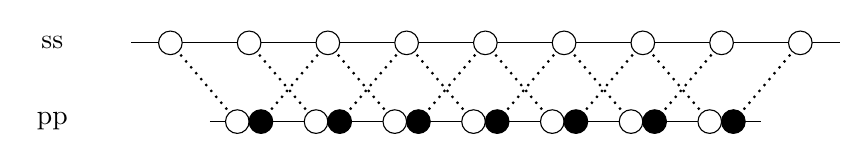
\begin{tikzpicture}
\node at (0.5,0){pp};
\node at (0.5,1){ss};
\draw (1.5,1)--(10.5,1);
\draw (2.5,0)--(9.5,0);
\foreach\x in {2,3,...,8}{
	\draw[dotted,thick] (\x,1)--++(0.85,-1);
	\draw[dotted,thick] (\x+2,1)--++(-0.85,-1);
	\draw[fill=white] (\x,1) circle (0.15cm);
	\draw[fill=white] (\x+0.85,0) circle (0.15cm);
	\draw[fill=black] (\x+1.15,0) circle (0.15cm);
}
\draw[fill=white] (9,1) circle (0.15cm);
\draw[fill=white] (10,1) circle (0.15cm);
\end{tikzpicture}
\end{center}
at $k=\pi/a$, the orbitals are made up of $\phi_r$'s with alternating coefficents (real part), and the interactions look like follows
\begin{center}
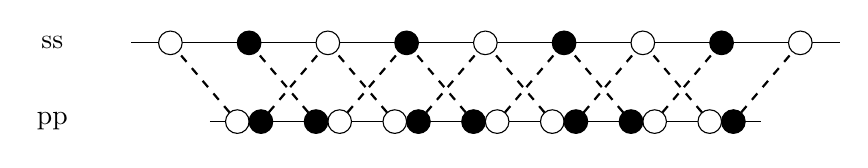
\begin{tikzpicture}
\node at (0.5,0){pp};
\node at (0.5,1){ss};
\draw (1.5,1)--(10.5,1);
\draw (2.5,0)--(9.5,0);
\foreach\x in {2,3,...,8}{
	\draw[dashed,thick](\x,1)--++(0.85,-1);
}
\foreach\x in {4,5,...,10}{
	\draw[dashed,thick](\x,1)--++(-0.85,-1);
}
\foreach\x in {2,4,...,8}{
	\draw[fill=white] (\x,1) circle (0.15cm);
	\draw[fill=black] (\x+1,1) circle (0.15cm);
}
\draw[fill=white] (10,1) circle (0.15cm);
\foreach\x in {3,5,7,9}{
	\draw[fill=white] (\x-0.15,0) circle (0.15cm);
	\draw[fill=black] (\x+0.15,0) circle (0.15cm);
}
\foreach\x in {4,6,8}{
	\draw[fill=white] (\x+0.15,0) circle (0.15cm);
	\draw[fill=black] (\x-0.15,0) circle (0.15cm);
}
\end{tikzpicture}
\end{center}
Clearly, half the interactions are constructive and half are destructive, so there's overall no net mixing.
\paragraph{The case of $k=\pi/2a$}
At $k=\pi/2a$, the coefficients cycle in $\{1,0,-1,0\}$, so we have the following interactions. Note that the diagram is drawn by taking the real part of the ss band and the imaginary part of the pp band\footnote{This is justified by thinking about the actual integral in the secular equation, which is \hl{incomplete}}:
\begin{center}
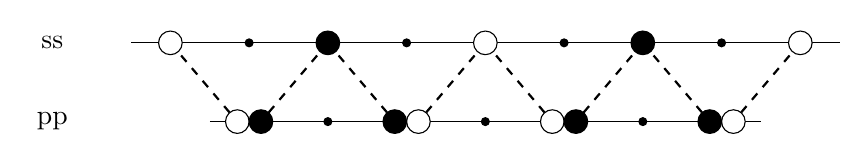
\begin{tikzpicture}
\node at (0.5,0){pp};
\node at (0.5,1){ss};
\draw (1.5,1)--(10.5,1);
\draw (2.5,0)--(9.5,0);
\foreach\x in {2,4,6,8}{
	\draw[dashed,thick] (\x,1)--++(0.85,-1);
	\draw[dashed,thick] (\x+2,1)--++(-0.85,-1);
}
\foreach\x in {2,6,10}{
	\draw[fill=white] (\x,1) circle (0.15cm);
}
\foreach\x in {4,8}{
	\draw[fill=black] (\x,1) circle (0.15cm);
}
\foreach\x in {3,7}{
	\draw[fill=white] (\x-0.15,0) circle (0.15cm);
	\draw[fill=black] (\x+0.15,0) circle (0.15cm);
}
\foreach\x in {5,9}{
	\draw[fill=white] (\x+0.15,0) circle (0.15cm);
	\draw[fill=black] (\x-0.15,0) circle (0.15cm);
}
\foreach\x in {3,5,7,9}{
	\draw[fill=black] (\x,1) circle (0.05cm);
}
\foreach\x in {4,6,8}{
	\draw[fill=black] (\x,0) circle (0.05cm);
}
\end{tikzpicture}
\end{center}
In summary, mixing does not happen at $k=0$ or $k=\pi/a$, the band boundary, and is strongest at $k=\pi/2a$.
\subsection{Hybrid orbital bases}
Instead of mixing $s$ and $p$ orbitals after formation of crystal orbitals, we can just hybridise them first. We follow the following guidelines
\begin{enumerate}
	\item Form left and right pointing arrays of HAOs in the same phase
	\item Overlap these constructively and destructively into $\sigma$ and $\sigma^*$
	\item \hl{incomplete}
\end{enumerate}
\subsection{Two-orbital bases}
\hl{incomplete}






\section{Semiconductors}


\subsection{Properties of intrinsic semiconductors}
Classic intrinsic semiconductors include Group 14 elements such silicon and germanium, which are tetrahedral solids. The bonding is much the same as discussed in 1D, with neighbouring $sp^3$ hybrids forming $\sigma$ and $\sigma^*$ MOs, the neighbouring MOs then interact to form bands, as shown below
\begin{center}
\begin{tikzpicture}[scale=1.5]
\node[font=\footnotesize, text width=1.5cm,align=center] at (0.5,2.0){Degenerate\\HAOs};
\node[font=\footnotesize, text width=1.5cm,align=center] at (2.0,2.0){$\sigma$ and $\sigma^*$\\MOs};
\node[font=\footnotesize, text width=3cm,align=center] at (3.5,2.0){$\sigma$ band (VB)\\and $\sigma^*$ band (CB)};
\draw[dashed] (1,0)--(1.5,1);
\draw[dashed] (1,0)--(1.5,-1);
\draw[dashed] (2.5,1)--(3.0,1.5);
\draw[dashed] (2.5,1)--(3.0,0.5);
\draw[dashed] (2.5,-1)--(3.0,-1.5);
\draw[dashed] (2.5,-1)--(3.0,-0.5);
\draw[{Stealth}-{Stealth}](3.5,-0.5)--node[right,font=\footnotesize]{$E_{\mathrm{g}}$}(3.5,0.5);
\draw[{Stealth}-{Stealth}](2,-0.97)--node[right,font=\footnotesize]{$2|\beta|_1$}(2,0.97);
\draw[{Stealth}-{Stealth}](4.1,0.5)--node[right,font=\footnotesize]{$2|\beta|_2$}(4.1,1.5);
\draw[{Stealth}-{Stealth}](4.1,-0.5)--node[right,font=\footnotesize]{$2|\beta|_2$}(4.1,-1.5);
\draw[fill=gray!50!black] (0,-0.06) rectangle (1,+0.06);
\draw[fill=white] (1.5,0.97) rectangle (2.5,1.03);
\draw[fill=black] (1.5,-0.97) rectangle (2.5,-1.03);
\draw[fill=white] (3.0,0.5) rectangle (4.0,1.5);
\draw[fill=gray!60!white] (3.0,-0.5) rectangle (4.0,-1.5);
\end{tikzpicture}
\end{center}
On descending Group 14, $|\beta|_1$, which results from overlap of the directly pointing hybrids, decrease in magnitude, as the orbitals become more diffuse; however $|\beta|_2$ which is proportional \hl{how?} to $\alpha_p-\alpha_s$, becomes larger as the $s$-$p$ separation increases down the group. The overall result is that the \emph{band gap decreases down the group}:
\begin{center}
	\begin{tabular}{cccccc}
	\hline
	 & Diamond & Si & Ge & $\alpha$-Sn & Pt\\
	 \hline
	 $E_{\mathrm{g}}$ (eV) & 5.3 & 1.14 & 0.67 & 0.08 & Not tetrahedral\\
	 \hline
	\end{tabular}
\end{center}
Note lead is not tetrahedral due to the high promotion energy to form hybrids.


\subsubsection{Conductivity}
\paragraph{Definitions}
\begin{itemize}
	\item \textbf{Resistivity} is the inherent property of a material $\rho=RA/l$, with units of $\Omega$ m.\par
	\item \textbf{Conductance} is the reciprocal resistance, $G=1/R$, with units of Siemens, S, which is equivalent of $\Omega^{-1}$.\par
	\item \textbf{Conductivity} is the reciprocal resistivity, $\sigma=1/\rho=Gl/A$, with units of S m$^{-1}$.\par
\end{itemize}
Conductivity is governed by the equation
\begin{equation}
	\sigma=n_{\mathrm{e}}e\mu_{\mathrm{e}}+n_{\mathrm{h}}e\mu_{\mathrm{h}}
\end{equation}
where the $\mu_i$'s are again not permittivity constants but \emph{mobility} of electrons and holes. In an intrinsic semiconductor, the number of electrons is exactly equal to to the number of holes, so conductivity is directly proportional to the number of CB electrons, $N_{\mathrm{e}}$. We can evaluate $N_{\mathrm{e}}$ by integrating over energy $E$the density of \emph{occupied} states, which is simply the density of states superimposed on the Fermi-Dirac distribution: $Z(E)=f(E)\times D(E)$:
\begin{subequations}
\begin{align}
N_{\mathrm{e}}&=\int^{\inf}_{E_{\mathrm{c}}}f(E)\times D(E)\dif E\\
&=\int^{\inf}_{E_{\mathrm{c}}}\frac{1}{e^{(E-E_{\mathrm{F}})/kT}+1}\times D(E)\dif E\\
&\approx\int^{\inf}_{E_{\mathrm{c}}}e^{-(E-E_{\mathrm{F}})/kT}\times c\dif E\label{sigma3}\\
&=ckTe^{-(E_{\mathrm{c}}-E_{\mathrm{F}})/kT}\\
&\approx ckTe^{-E_{\mathrm{g}}/2kT}\label{sigma5}
\end{align}
\end{subequations}
where in \cref{sigma3} we used the fact that $(E_{\mathrm{c}}-E_{\mathrm{F}})\gg kT$, so the extra $+1$ can be ignored in the denominator; and also that the form of $D(E)$ can be approximated to a constant $c$ as the Fermi-Dirac distribution goes to zero so fast that the exact form of $D(E)$ matters little. And in \cref{sigma5} we used the fact that $(E_{\mathrm{c}}-E_{\mathrm{F}})=E_{\mathrm{g}}/2$ if the density of states for both bands are the same (which is likely since we're dealing with intrinsic semiconductors now.). The pre-exponential term is $ckT$, but the linear term is expected to be overwhelmed by the exponential quickly so is ignored. The main result is just that the activation energy for conductivity is approximately half of band gap
\begin{thrm}[Dependence of conductivity on temperature]
For an intrinsic semiconductor with a band gap $E_{\mathrm{g}}$, the conductivity is
\begin{equation}
	\sigma\propto e^{-E_{\mathrm{g}}/2kT}
\end{equation}
\end{thrm}
\subsubsection{Effective masses}
The tight-binding model essentially decouples $k$ from momentum, which allowed us to predict the movements of electrons in the FEG model, but clearly when a semiconductor becomes either thermally activated, or as we'll later see, doped, conduction can happen and we need to predict that within the tight-binding paradigm. To do that, we introduce the concept of \emph{effective mass}:
\begin{defi}[Effective mass]
The effective mass is the mass that an electron would need to have such that it responds to an applied field in the same way as an electron with the same $k$ value in the FEG model. The effective mass is related to the mobility $\mu$ of the electron. It is given as 
\begin{equation}
	\frac{1}{m_{\mathrm{e}}^*}=\frac{1}{\hbar^2}\diff[2]{E_k}{k}
\end{equation}
where $E_k$ is the dispersion relation yielded by the tight-binding model.
\end{defi}
So for our simple ss-$\sigma$ type band, the effect mass would be
\begin{equation}
	m_{\mathrm{	e}}^*=-\frac{\hbar^2}{2\beta a^2}\sec{ka}
\end{equation}
The relevant charge carriers for a semiconductor would be the holes near the top of the valence band and the electrons near the bottom of the conduction band, and
\begin{itemize}
	\item Holes near the top of the valence band have that $k\approx\pi/a$, so $m_{\mathrm{e}}^*<0$, but since holes have positive charges, they respond to applied fields the opposite way, so $m_{\mathrm{h}}^*$ is usually \emph{positive}.
	\item Electrons near the bottom of the conduction band have that $k\approx0$, so $m_{\mathrm{e}}^*>0$.
\end{itemize}
Basically, for most relevant cases, the \emph{effective masses of both electrons and holes are positive}.